\documentclass{article}
\usepackage[utf8]{inputenc}
\usepackage{graphicx}

\title{Lab1}
\author{Ballarin Simone }
\date{March 2019}

\begin{document}


\maketitle

\section{Domanda 1}
Il grafo reale era formato da un numero di nodi pari a 6474, inoltre vi erano presenti circa 13000 archi. Il grafo fornito era non orientato. 
Ci viene richiesto di generare grafi casuali con medisime caratteristiche di cardinalitlà del grafo reale utilizzando gli algoritmi ER e UPA.
Al fine di attuare la richiesta abbiamo dovuto calcolare la probabilità p per l'algoritmo ER, mentre il parametro m dell'algoritmo UPA è stato fornito nella domanda stessa.
La probabilità p è stata calcolata come segue:
Sia X una variabile aleatoria come segue X=Bin((n*(n-1)/2,p), questa varibile descrive il numero di successi dell'algoritmo ER (archi scelto), il quale effettua n*(n-1)/2 scelte che rappresenano la creazione di un arco tra due nodi non identici con probabilita' p ignota.
Volendo avere una media di archi generati da ER pari a quella del grafico reale (che significa E(X)=13xxx) e inoltre sapendo E(X)=n*(n-1)/2*p, possiamo dedurre p=13xxx/n*(n-1)*2.

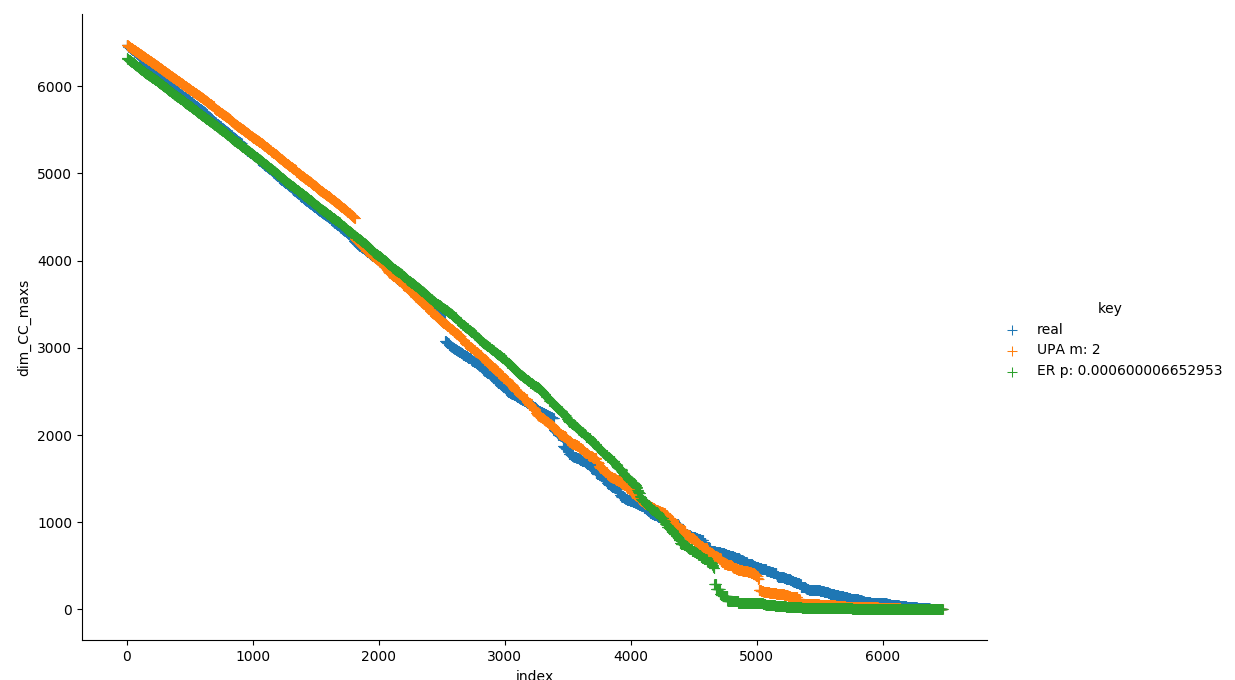
\includegraphics[width=0.9\textwidth]{Figure_4}

\newpage
\section{Domanda 2}
Al fine di valutare i comportamenti dei tre grafi ad un attacco casuale abbiamo inserito nel grafico due rette: quella orizzonatale corrispondete al limite di resilienza del 75\% (4576 nodi); mentre la retta verticale indica il superamento del 20\% (1295 nodi) dei nodi rimossi. 
Osservando i tre gruppi di punti rispetto a queste due rette nella prima figura, si può osservare che dopo aver rimosso il 20\% dei nodi tutte e tre i grafi sono oltre il limite di resilienza fissato al 75\%, con il grafo UPA in leggere vantaggio, mentre ER e quello reale presentano differenze non apprezzabili.
Il test è stato rieffettuato e nella seconda figura si presentano i risultati. Si può notare come anche in questo caso tutti i tre grafi dopo l'eliminazine del 20\% dei nodi si presentino praticamente con lo stessa resilienza.
In conclusione notiamo che i gruppi di punti sono essenzialmente comparabili, l'unica differenza riscontrabile si puo' apprezzare nella parte finale dell'asse orrizzontale in cui le varie resilienze si discostano.

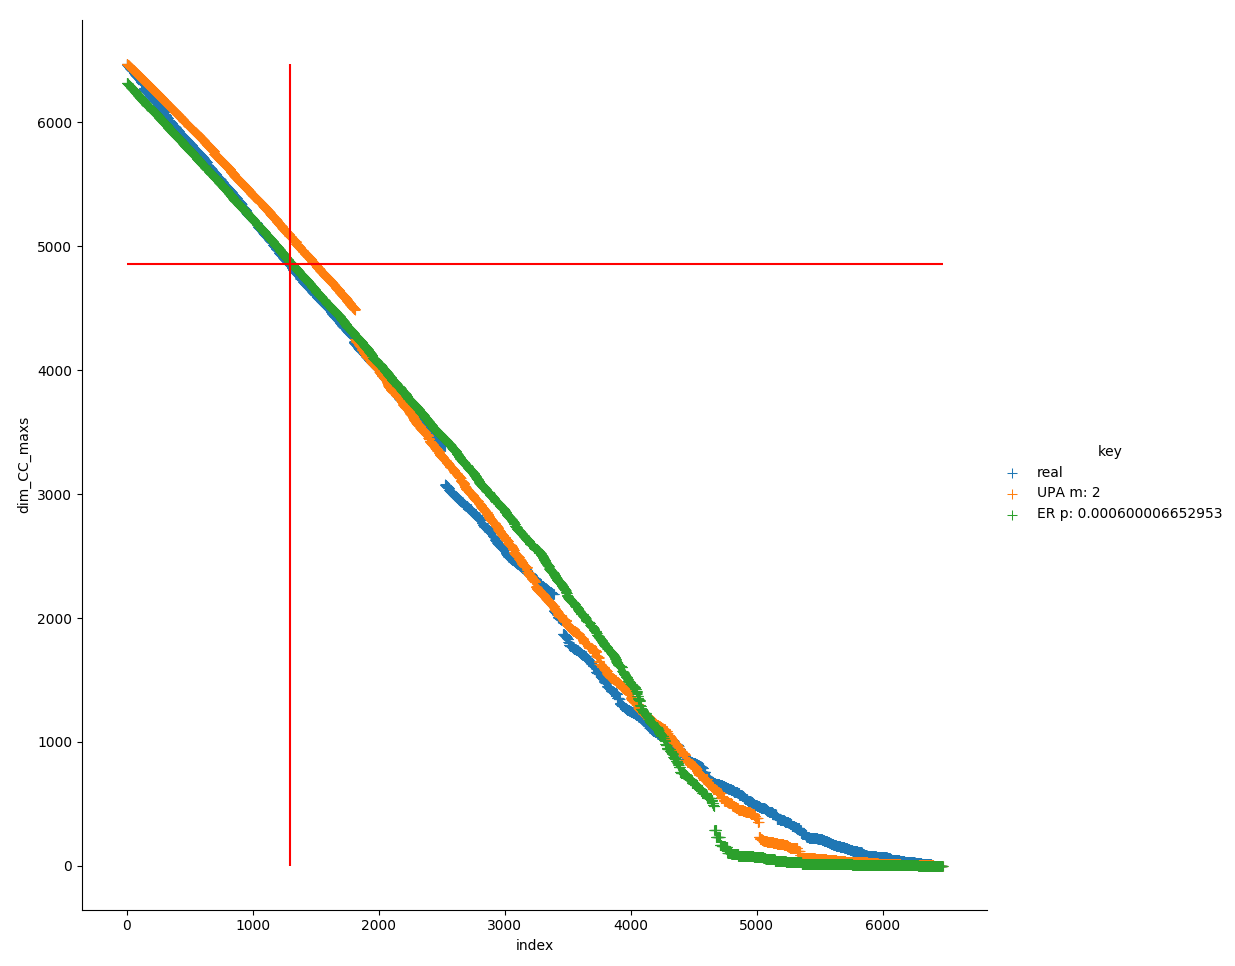
\includegraphics[width=0.9\textwidth]{Figure_2}

\section{Domanda 3}
Abbiamo effettuato l'attacco con strategia max-degree. Il seguente grafico presenta la correlazione tra nodi rimossi e dimensione della componente massima come richiesto dalla domanda.

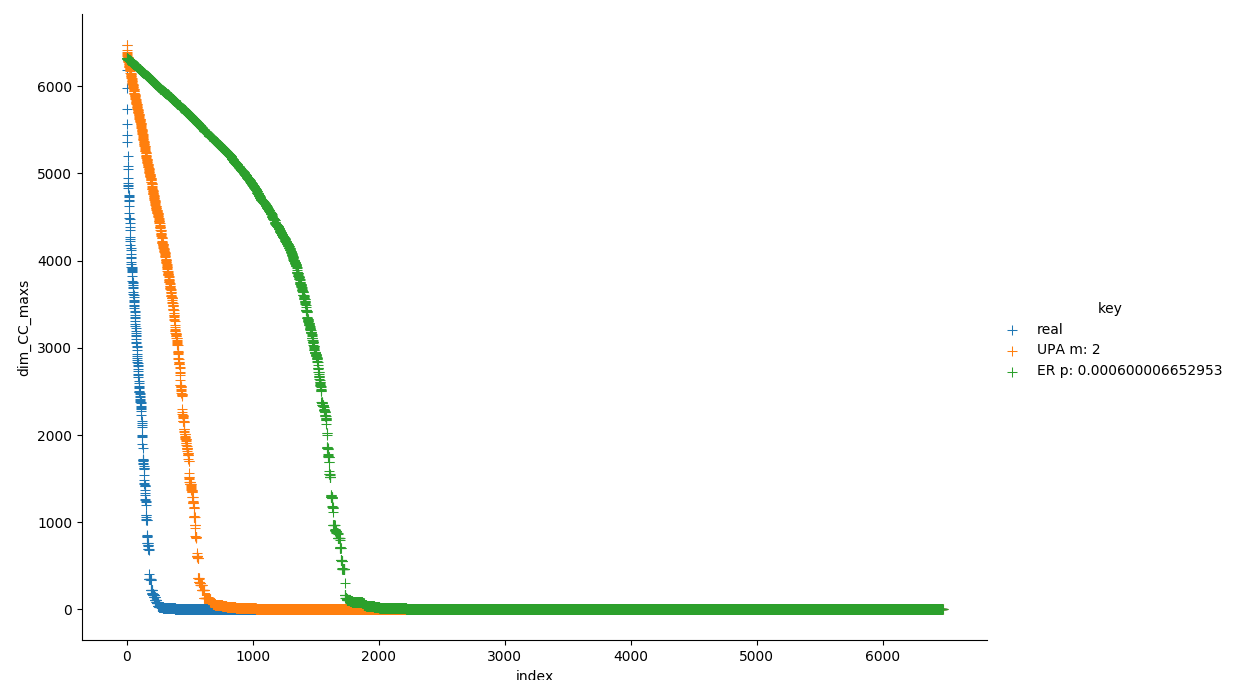
\includegraphics[width=0.9\textwidth]{Figure_3}

\section{Domanda 4}
In maniera analoga a quanto fatto ai grafici esposti in domanda 2, si e' insirita una retta per il limite di resilienza al 75\% e una per il superamento del 20\% dei nodi rimossi.
In questo caso tutti i grafi sono sotto la soglia di resilienza, però stavolta presentano andamenti estremamente differenti.
Il grafo reale e' quello che si comporta peggio: come si puo' notare ha una caduta repentina gia' dopo le prime rimozioni e dopo circa 200 rimozione ha relienza quasi nulla.
Il grafo UPA invece ha una caduta meno violenta comporata al grafo reale, ma comunque veloce. La resilienza si annulla quasi completamente gia' dopo 700 rimozioni.
Il grafo ER risulta invece quello piu' resistenza: nonostante non riesca a mantenersi sopra la soglia dopo il 20\$ delle rimozioni e' quello che si avvicina maggiormente. Fino a quasi 1000 rimozioni tiene un decrescita quasi lineare, mentra tra 1000 e 1200 rimozioni il tasso di decrescita aumenta fino a diventa circa esponenziale dopo il limite delle 1200 rimozioni.\\
Queste differenze le imputiamo alle diverse topologie che i vari grafi prentano. Queste infatti essendo che la scelta non e' piu' casuale influenzano gli effetti dei vari attacchi.\\
ER avendo una varianza del grado piu' bassa rispetto agli altri e' quello che si comporta meglio; UPA invece per come lavora l'algoritmo tende a creare pochi nodi con grado alto e tanti nodi con grado basso che si collegano a questi, l'attacco intelligente rimuovendo per i pchi nodi a grado alto ottiene dei buoni risultati nell'abbassamento della resilienza.
Il grafo reale, invece, intuiamo essere caratterizzato da un basso numero di nodi ad alto grado (le citta' piu' importanti) alle quali sono collegati un numero limitato di nodi di grado basso (la periferia della citta'). A differenza di UPA questi nodi di grado alto non sono collegati a meno nodi (per motivi geografici) e quindi per questa ragione presenta una robustezza inferiore.

Al fine di avere una maggiore comprensione della topologia abbiamo deciso di realizzare tre rappresentazioni grafiche dei vari grafi. Si rappresentano i nodi con cerchi di raggio proporzionale al grado.

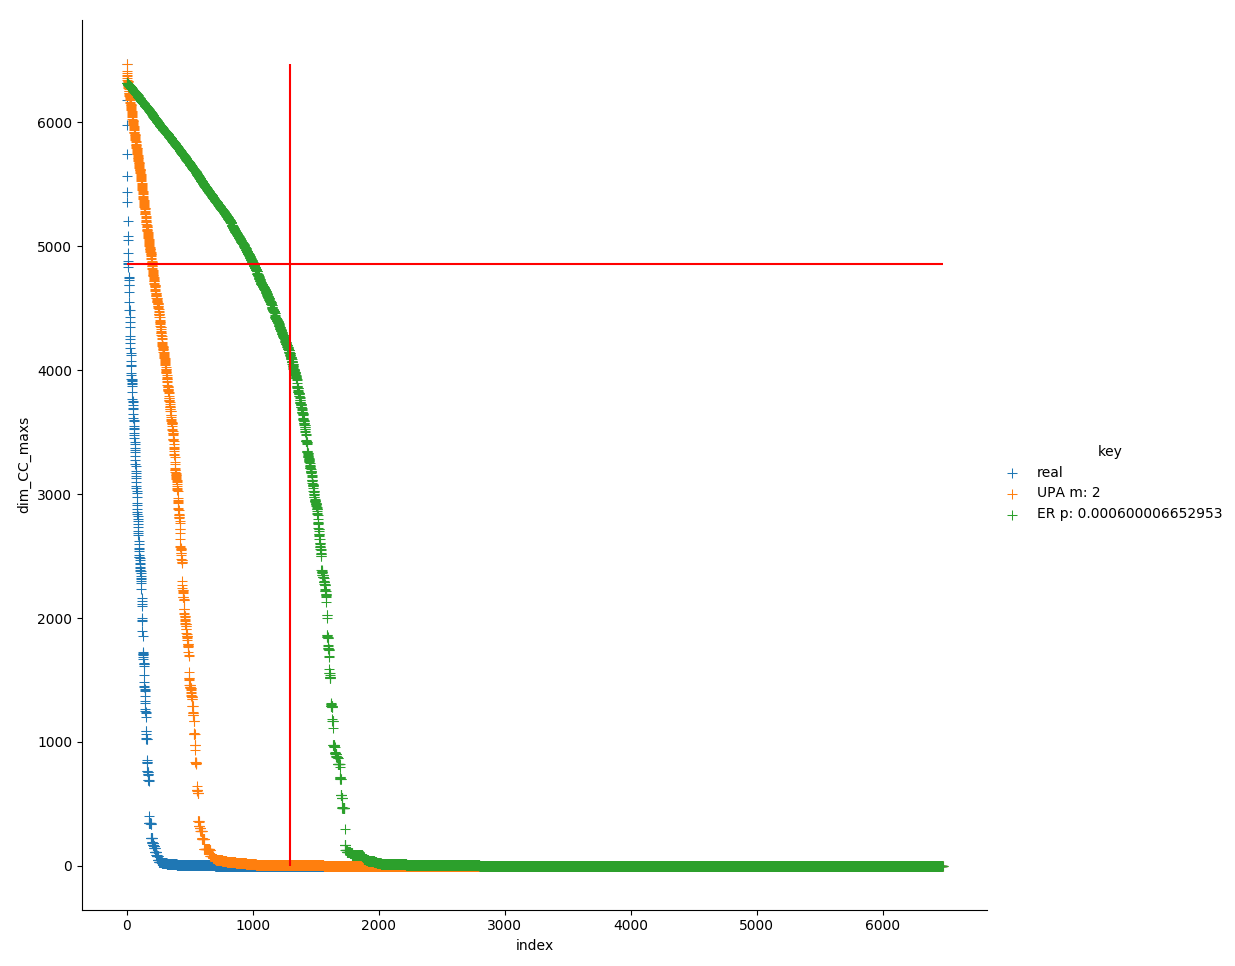
\includegraphics[width=0.9\textwidth]{Figure_1}

\section{Domanda 5}
In allegata alla consegna sono stati inseriti i codice sorgenti python dei vari file.
    
\end{document}
